\documentclass[aspectratio=169]{beamer}
\geometry{paperwidth=160mm,paperheight=100mm}
\usepackage{beamerthemesidebar}
\usepackage{hyperref}
\usepackage{color}
\usepackage{multimedia}
\usepackage{colortbl}
\usepackage{amsmath}
\usepackage{empheq}
\usepackage{cancel}
\usepackage{amssymb}
\usepackage{amsfonts}
\usepackage{lipsum}
\usepackage{tcolorbox}
\usepackage{tabularx}
\usepackage{caption}
\usepackage{bm}

\setbeamersize{sidebar width right=0pt}
\setbeamertemplate{footline}[frame number]
%
\definecolor{orange}{RGB}{250,167,12}
\definecolor{yellow}{RGB}{246,250,12}
\definecolor{green}{RGB}{128,238,1}
\definecolor{black}{RGB}{0,0,0}
\definecolor{blue}{RGB}{0,0,255}
\definecolor{red}{RGB}{255,0,0}
\definecolor{sepia}{RGB}{94,38,18}
\newcommand{\ve}[1]{{\rm\bf {#1}}}
\newcommand{\q}[1]{\textcolor{blue}{#1}}
\newcommand{\blue}[1]{\textcolor{blue}{#1}}
\newcommand{\sepia}[1]{\textcolor{sepia}{#1}}
\newcommand{\red}[1]{\textcolor{red}{#1}}
\newcommand{\green}[1]{\textcolor{green}{#1}}
\newcommand{\yellow}[1]{\textcolor{yellow}{#1}}
\newcommand{\orange}[1]{\textcolor{orange}{#1}}
\definecolor{burlywood}{RGB}{255,211,155}
\definecolor{chocolate}{RGB}{255,127,36}
\definecolor{tan}{RGB}{210,180,140}
%
\def\onethird{{\textstyle{1\over3}}}
\def\twothirds{{\textstyle{2\over3}}}
\def\fourthirds{{\textstyle{4\over3}}}
\def\onehalf{{\textstyle{1\over2}}}
\def\threehalfs{{\textstyle{3\over2}}}
%
\newcommand{\pd}{\partial}
\newcommand{\aMLT}{\alpha_{\rm MLT}}
\newcommand{\Fconv}{F_{\rm conv}}
\newcommand{\Frad}{F_{\rm rad}}
\newcommand{\Ftot}{F_{\rm tot}}
\newcommand{\Hp}{H_p}
\newcommand{\prad}{p_{\rm rad}}
\newcommand{\pgas}{p_{\rm gas}}
\newcommand{\TTc}{T_{\rm c}}
\newcommand{\rhoc}{\rho_{\rm c}}
\newcommand{\Teff}{T_{\rm eff}}
\newcommand{\Fstar}{F_\star}
\newcommand{\pstar}{p_\star}
\newcommand{\Pstar}{P_\star}
\newcommand{\Rstar}{R_\star}
\newcommand{\rhostar}{\rho_\star}
\newcommand{\Tstar}{T_\star}
%
\title{Theoretical Astrophysics I: Physics of Sun and Stars\\
Lecture 13: Quiz!!!}
\author{\texorpdfstring{\sepia{Petri K\"{a}pyl\"{a} Ivan Mili\'{c}}\newline\blue{\url{pkapyla, milic@leibniz-kis.de}}}{}}
\institute{Institut f\"ur Sonnenphysik - KIS, Freiburg}
\date{\today}
%
\begin{document}
\frame{\titlepage}


%
\frame{
\frametitle{What are we doing today?}
\begin{itemize}
\item This will be a set of short questions, numerical problems, theoretical / conceptual questions to test what you remembered and help you prepare for the exam.
\item You can expect that the problems at the exam will be somewhat more specific. 
\end{itemize}
}
%
%
\frame{
\frametitle{Question 1:}
If a star is in hydrostatic equilibrium, what two forces are in balance? Derive the appropriate expression.
}
%
%
\frame{
\frametitle{Question 2:}
\begin{minipage}{0.54\linewidth}
On the given HR diagram, mark the stars that belong to the main sequence, red giants and white dwarves. 
\end{minipage}
\begin{minipage}{0.45\linewidth}
%\begin{figure}
%PJK: file doesn't exit
%  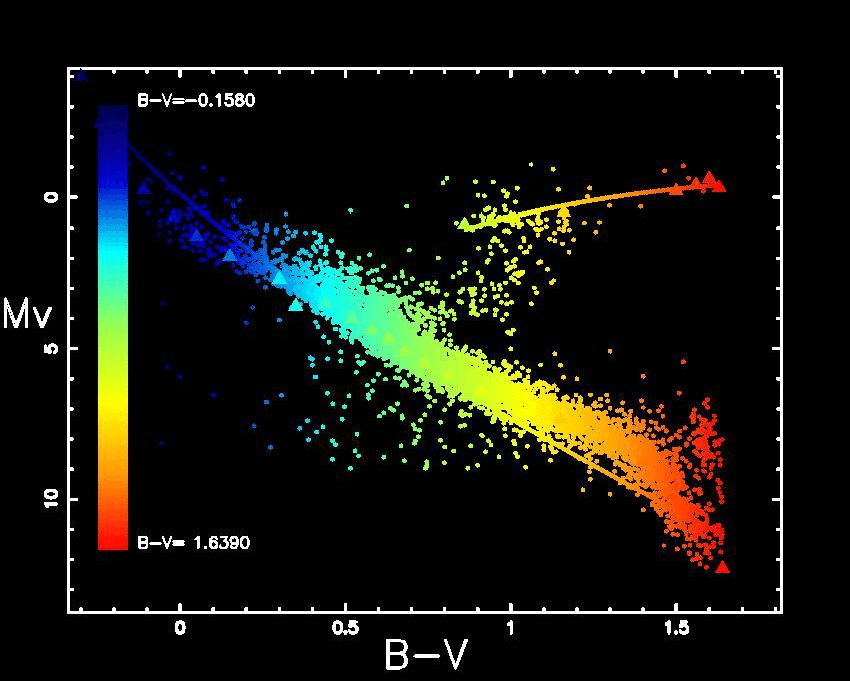
\includegraphics[width=6cm]{figures/hr.png}
%\end{figure}
\end{minipage}
}
%
\frame{
\frametitle{Question 3:}
If a blue giant and a red giant star have the same absolute brigthness, and blue giant has effective temperature of 20\,000\,K, while the red giant has effective temperature of 3\,000\,K - how do their radii relate?
}
%
\frame{
\frametitle{Question 4:}
Write down the equation of state (relationship between pressure, density and temperature) for a gas that only consists of Hydrogen and Helium and is: a) completely ionized; b) completely neutral
}
%
%
\frame{
\frametitle{Question 5:}
Recall the homology relationship between the mass and luminosity of the main sequence stars. What can it tell us about the dependence of the star lifetime on its mass? Which stars live longer, stars of high mass or low mass?
}
%
\frame{
\frametitle{Question 6:}
Explain briefly why a red giant phase lasts much shorter than the main sequence phase. 
}
%
\frame{
\frametitle{Question 7:}
Related to the previous question - how come that we see so many giants then? 
}
%
\frame{
\frametitle{Question 8:}
Explain the conceptual difference between convective and radiative energy transport. 
}
%
\frame{
\frametitle{Question 9:}
Starting from the radiative transfer equation:
\begin{equation}
\cos \theta \frac{dI_\nu}{\rho dz} = - \kappa_\nu I_\nu + j_\nu
\end{equation}
show that the radiative flux is proportional to the gradient of temperature and inversely proportional to the mean opacity $\overline{\kappa}$
}
\frame{
\frametitle{Question 10:}
%
Name the three most important nuclear reactions / chains of nuclear
reactions occurring in main sequence stars. In what kinds of stars do
they occur?
%
}
%
\frame{
\frametitle{Question 11:}
%
Describe shortly what are the end states of stars with $0.3$, $1$ and
$20$ solar masses? Explain why.
%
}
%
%
\frame{
\frametitle{Question 12:}
%
Stellar structure models are one dimensional and consider all
quantities to depends on radius only. Why is this a good approximation
for most stars? When is one-dimensionality no longer a good
approximation?
%
}
%
\frame{
\frametitle{Question 13:}
%
There are three evolutionay timescales that arise from the equations
of stellar structure. What are they and what do they describe?
Describe an evolutionary stage where a star evolves in each one the
timescales.
%
}
%
%
\frame{
\frametitle{Question 14:}
%
Why does convection (heat transport by fluid motions) occur? Name two
physical situations where convection ensues and describe in which kind
of stars such situations occur.
%
}
%
\frame{
\frametitle{Question 15:}
%
Explain what the Chandrasekhar mass is and what happens if it is
exceeded.
%
}
%
\frame{
\frametitle{Question 16:}
%
What are Cepheids and why are they important for astrophysics?
%
}
%
\frame{
\frametitle{Question 17:}
%
Name two methods how can you estimate the masses of stars from
observations.
%
}
%
\frame{
\frametitle{Question 18:}
%
What is a black body and why you can approximate stars to be black
bodies?
%
}
%
\frame{
\frametitle{Question 19:}
%
Name the equations of state that can be used describe the gas in
stellar interiors and give examples of star / evolutionary phases
where each one is dominant.
%
}
%
\frame{
\frametitle{Question 20:}
%
How can you determine the ages of stars?
%
}
%
\end{document}


